\documentclass[pdftex,12pt,a4paper]{article}

\usepackage{graphicx}  
\usepackage[margin=2.5cm]{geometry}
\usepackage{breakcites}
\usepackage{indentfirst}
\usepackage{pgfgantt}
\usepackage{pdflscape}
\usepackage{float}
\usepackage{epsfig}
\usepackage{epstopdf}
\usepackage[cmex10]{amsmath}
\usepackage{stfloats}
\usepackage{multirow}
\usepackage{hyperref}



\renewcommand{\refname}{REFERENCES}
\linespread{1.3}

\usepackage{mathtools}
%\newcommand{\HRule}{\rule{\linewidth}{0.5mm}}
\thispagestyle{empty}
\begin{document}
\begin{titlepage}
\begin{center}
\textbf{}\\
\textbf{\Large{ISTANBUL TECHNICAL UNIVERSITY}}\\
\vspace{0.5cm}
\textbf{\Large{COMPUTER ENGINEERING DEPARTMENT}}\\
\vspace{2cm}
\textbf{\Large{BLG 242E\\ DIGITAL CIRCUITS LABORATORY\\ HOMEWORK 3}}\\
\vspace{2.8cm}
\begin{table}[ht]
\centering
\Large{
\begin{tabular}{lcl}
\textbf{HOMEWORK NO}  & : & 3 \\
\textbf{HOMEWORK DATE}  & : & 28.05.2023\\
\textbf{LAB SESSION}  & : & FRIDAY - 10.30 \\
\textbf{GROUP NO}  & : & G8 \\
\end{tabular}}
\end{table}
\vspace{1cm}
\textbf{\Large{GROUP MEMBERS:}}\\
\begin{table}[ht]
\centering
\Large{
\begin{tabular}{rcl}
150200919  & : & Abdullah Jafar Mansour Shamout \\
150220762  & : & Muhammed Yusuf Mermer  \\
\end{tabular}}
\end{table}
\vspace{2.8cm}
\textbf{\Large{SPRING 2023}}

\end{center}

\end{titlepage}

\thispagestyle{empty}
\addtocontents{toc}{\contentsline {section}{\numberline {}FRONT COVER}{}}
\addtocontents{toc}{\contentsline {section}{\numberline {}CONTENTS}{}}
\setcounter{tocdepth}{4}
\tableofcontents
\clearpage

\setcounter{page}{1}

\section{INTRODUCTION} 
In this experiment we implemented 2 designs of an 8-bit data bus using tristate buffers. We also implemented memory modules that can store 8-bits,8-bytes,32-bytes,128-bytes. We learned how to utilize the tristate buffer as an if statement and how it helps us in creating a bus. We also learned how to use the generate block to generate higher storage memory elements from lower ones.


\section{EXPERIMENT}
\subsection{Part 1}
In this experiment we implemented an 8-bit data bus with 2 drivers and one output. We needed to create a tristate buffer as a separate module to create the bus. We also used a select input to act as an enable to the buffers to decide which one outputs to the bus instead of using multiplexers.

\hyperlink{hype1}{See the result of this part}

\subsection{Part 2}

In this part, besides of the previously made 8 bit bus, we also defined 8 bit bus with 2 outputs. The only difference between former and later is after the tristate buffers in the second one, they are not connected to same output. Which makes one output always high impedance (Z) because just one of them at a time will be active. After we made relevant connections required for this question, we see that O1 shows D1 and Z, O2 shows D2 and Z. When O1 is Z, O2 is D2 and O1 is D1, O2 is Z depending on the S.

\hyperlink{hype2}{See the result of this part}


\subsection{Part 3}
In this experiment we implemented an 8-bit memory module that takes 8-bit input and outputs 8-bits, It also takes reset,read,write,clock inputs and select input which acts as an enable at this level. To achieve the required functionality for this module we had to create a storage register to store the 8-bits when needed and output it when needed. Also we utilized 3 always blocks as input being written is dependent on the positive clock edge, the reset happens on its negative edge, and reading is not dependent on anything according to the question so we used an asterisk (*) always condition to monitor it. If select and read are not both 1 instead of outputting the storage we output high impedance, which isn't very useful now, but will be once we use this module to create higher storage elements from this module if the output bus is of lower size than the storage elements.

\hyperlink{hype3}{See the result of this part}

\subsection{Part 4}
In this experiment we implemented an 8-byte memory module using the previous 8-bit memory module. A byte means 8-bits so 8 bytes would require us to call the module 8 times. To do this we utilized the generate block. Each module would take the same clock , input, read, write, and reset signals. However, for the select signal, since we will only activate one 8-bit module "Word" of this module, their select signals will be 0 for all of them except the one at the address signal specified to our 8-byte module. To achieve this I created an address table selection (ATS) wire, I assigned its value inside the generate block with a variable (i). Using this variable I assigned the ATS bit for that specific 8-bit module call by checking if its equal to the address or not, if it is then I assign a 1, if it is not, I assign a 0. I also ANDed the select with chipselect to make sure that the chip is selected as specified in the question. As for the outputs I connected them all to a O wire which acts as a bus since the non selected 8 bit memory modules will give high impedance.

\hyperlink{hype4}{See the result of this part}

\subsection{Part 5}
In this part of the question, we especially focused on the chip selection inputs arrived to 8 byte memories.  First two bits of address (in this situation 3 and 4) used to activate chip select. With the help of AND and NOT gates, we send a bit of information to all 8 byte memories in order to activate one of them. Other address bits (0 to 2) sent to all memories as address in order to detect the required line. Other types of inputs are directly sent to the memories because there is no other special case to deal with for these parameters. Outputs are connected to one line, because only one line comming from these memories will be the result we want and the others will be Z which don't have any effect on the circiut.

\hyperlink{hype5}{See the result of this part}

\subsection{Part 6}
In the last part, we again used 4 modules. However, for this time all 32 bytes modules are actively used. Due to an 32 byte module can only take and give 8 bit numbers, we at first separated input into 4 parts and send these 4 8 bits to different memories. Smiliar to the previous example, clock, adress, read, write and reset parameters are all as specified as in the previous parts so we did not make any specific implementation for these parameters and sent directly to the inputs of the 32 byte memories. Then we concatenated all the binary numbers according to the same order when we gave inputs.

\hyperlink{hype6}{See the result of this part}

\section{RESULTS}
\subsection{Schematics and Simulations}


\hypertarget{hype1}{}
\subsubsection{PART 1}


    \begin{figure}[H]
    	\centering
    	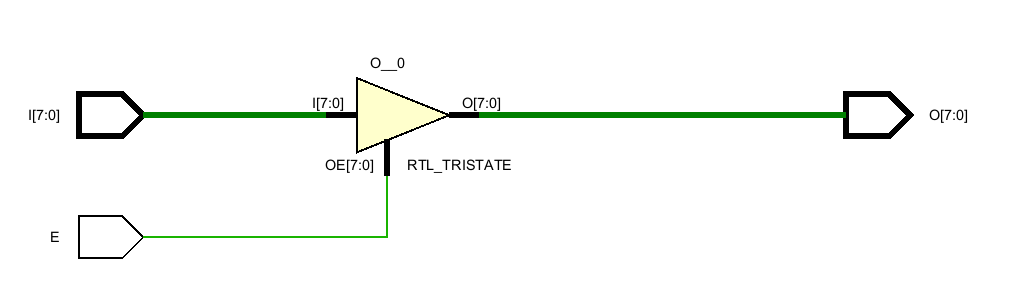
\includegraphics[width=0.8\textwidth]{schematic/buffer_schem.png}	
    	\caption{tristate buffer schematic}
    	\label{tristate buffer schematic}
    \end{figure}
    
    \begin{figure}[H]
    	\centering
    	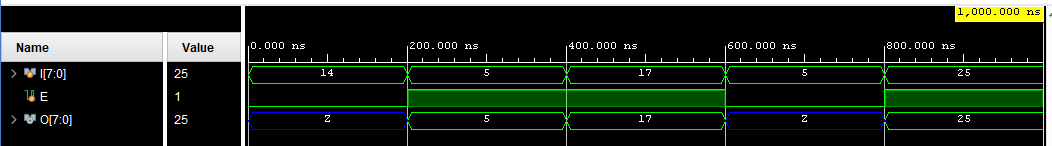
\includegraphics[width=1\textwidth]{simulations/buffer_sim.png}	
    	\caption{tristate buffer simulation}
    	\label{tristate buffer simulation}
    \end{figure}
    
    \begin{figure}[H]
    	\centering
    	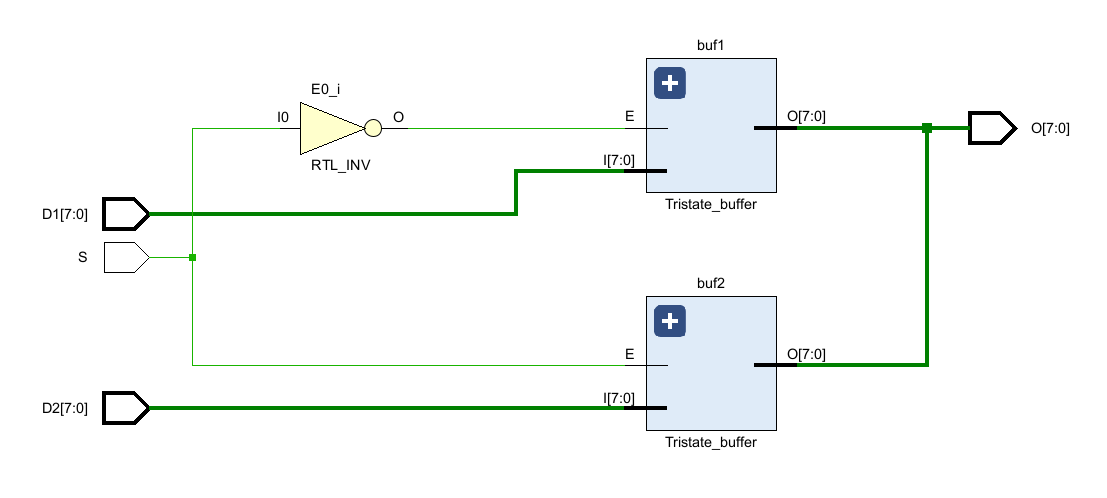
\includegraphics[width=0.8\textwidth]{schematic/bus_schem.png}	
    	\caption{1 output bus schematic}
    	\label{1 output bus schematic}
    \end{figure}
    
    \begin{figure}[H]
    	\centering
    	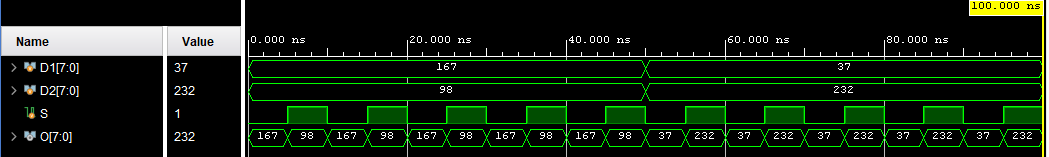
\includegraphics[width=1\textwidth]{simulations/bus_sim.png}	
    	\caption{1 output bus simulation}
    	\label{1 output bus simulation}
    \end{figure}
    


\hypertarget{hype2}{}
\subsubsection{PART 2}
\begin{figure}[H]
    	\centering
    	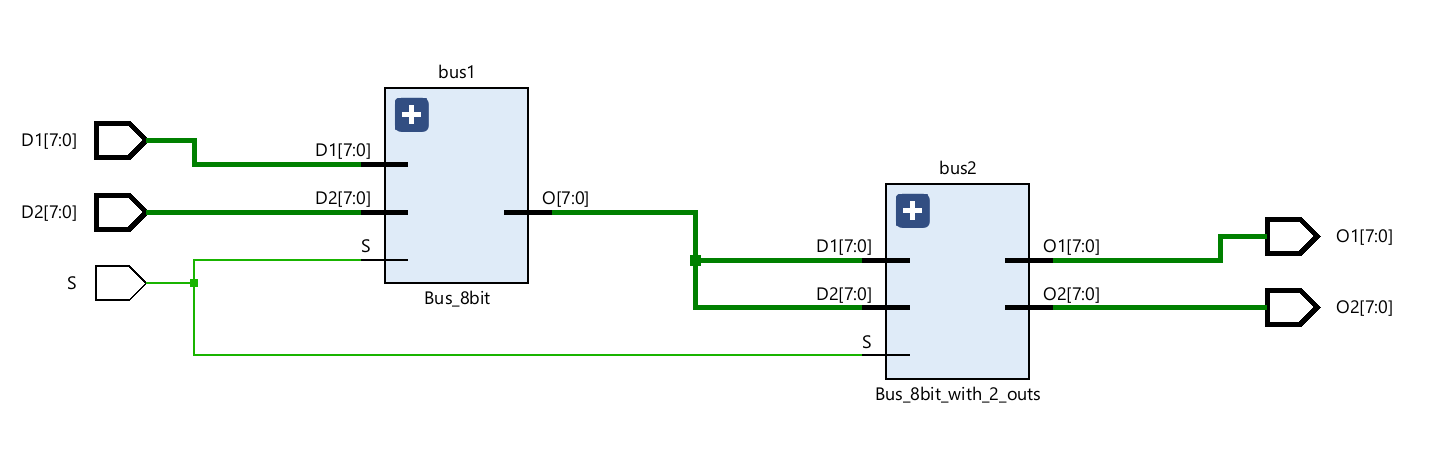
\includegraphics[width=1\textwidth]{schematic/part2_design.png}	
    	\caption{ 8-bit data bus with 2 drivers and 2 readers}
    	\label{ 8-bit data bus with 2 drivers and 2 readers}
    \end{figure}
    
    \begin{figure}[H]
    	\centering
    	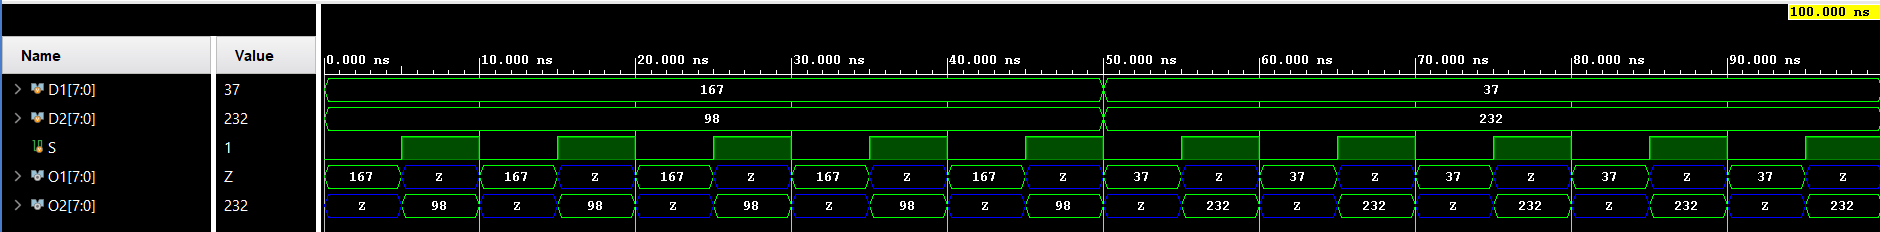
\includegraphics[width=1\textwidth]{simulations/part2_result.png}	
    	\caption{8-bit data bus with 2 drivers and 2 readers simulation}
    	\label{8-bit data bus with 2 drivers and 2 readers simulation}
    \end{figure}


\hypertarget{hype3}{}
\subsubsection{PART 3}
\begin{figure}[H]
    	\centering
    	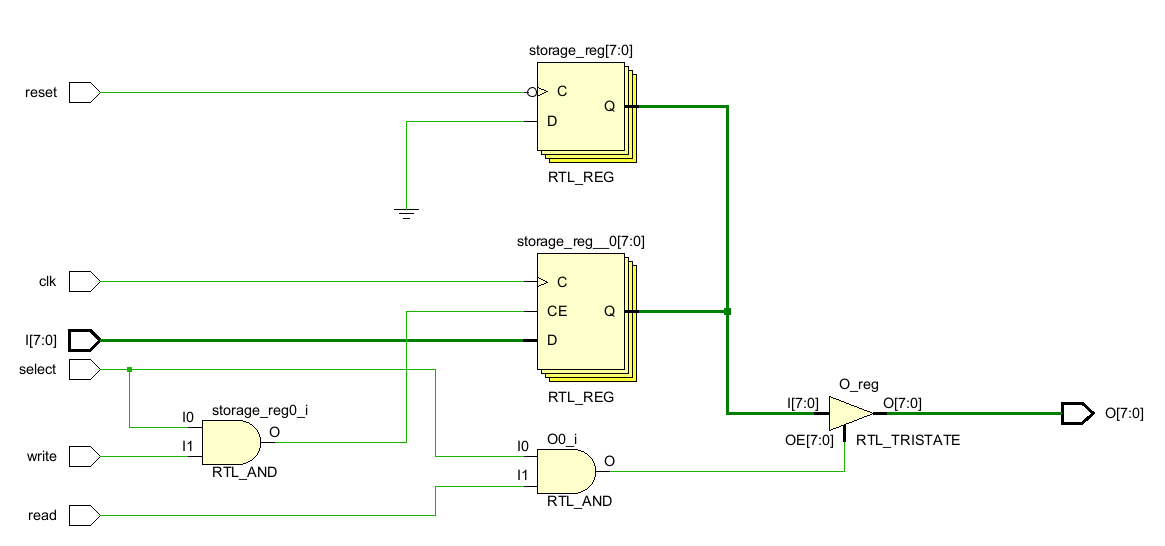
\includegraphics[width=0.8\textwidth]{schematic/8bit_schem.png}	
    	\caption{8-bit memory schematic}
    	\label{8-bit memory schematic}
    \end{figure}
    
    \begin{figure}[H]
    	\centering
    	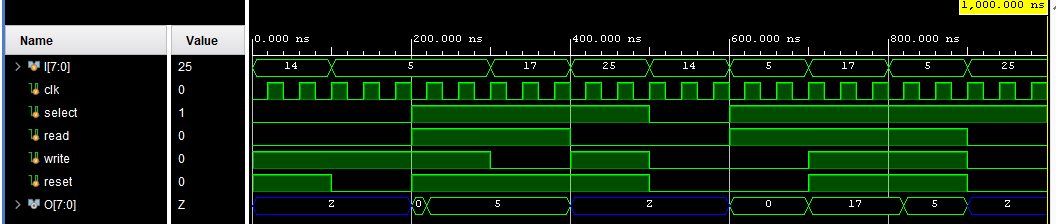
\includegraphics[width=1\textwidth]{simulations/8bit_sim.png}	
    	\caption{8-bit memory simulation}
    	\label{8-bit memory simulation}
    \end{figure}


\hypertarget{hype4}{}
\subsubsection{PART 4}

\begin{figure}[H]
    	\centering
    	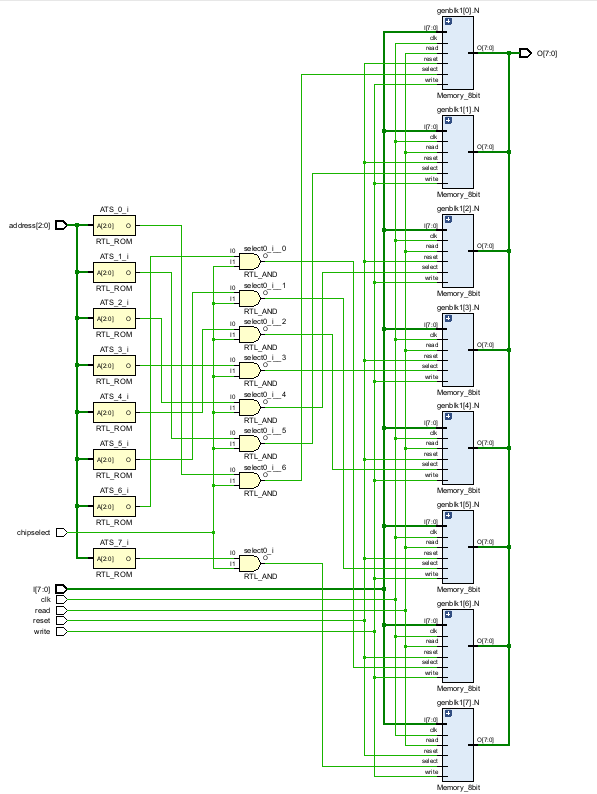
\includegraphics[width=0.8\textwidth]{schematic/8byte_schem.png}	
    	\caption{8-byte memory schematic}
    	\label{8-byte memory schematic}
    \end{figure}
    
    \begin{figure}[H]
    	\centering
    	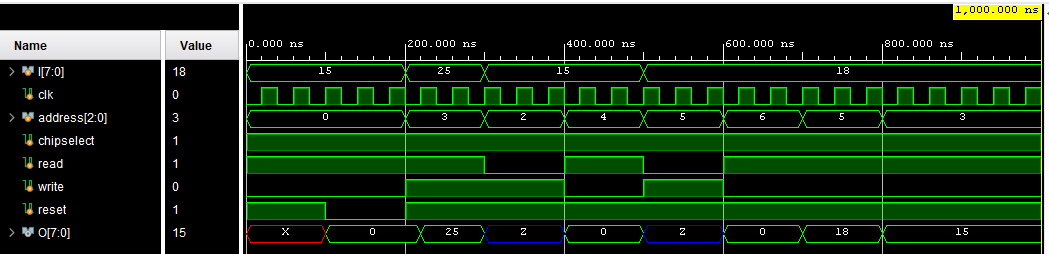
\includegraphics[width=1\textwidth]{simulations/8byte_sim.png}	
    	\caption{8-byte memory simulation}
    	\label{8-byte memory simulation}
    \end{figure}



\hypertarget{hype5}{}
\subsubsection{PART 5}

\begin{figure}[H]
    	\centering
    	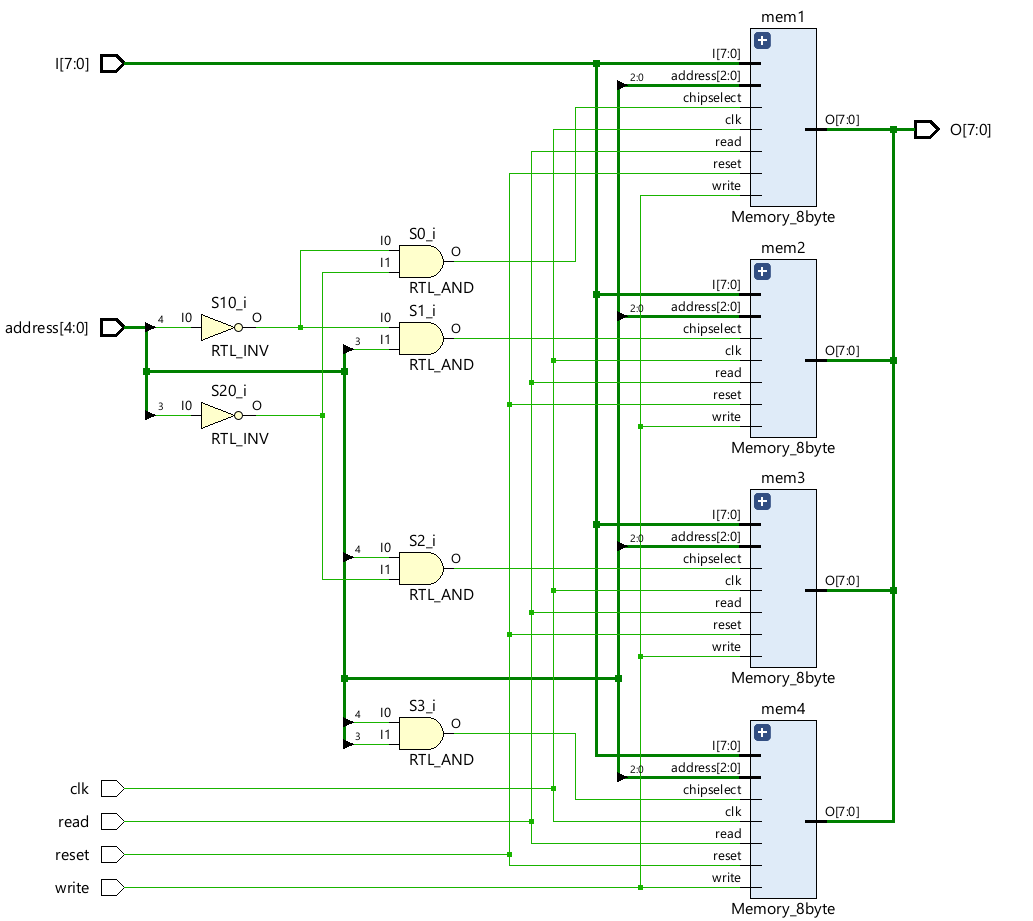
\includegraphics[width=0.8\textwidth]{schematic/part5_design.png}	
    	\caption{32 byte memory}
    	\label{32 byte memory}
    \end{figure}
    
    \begin{figure}[H]
    	\centering
    	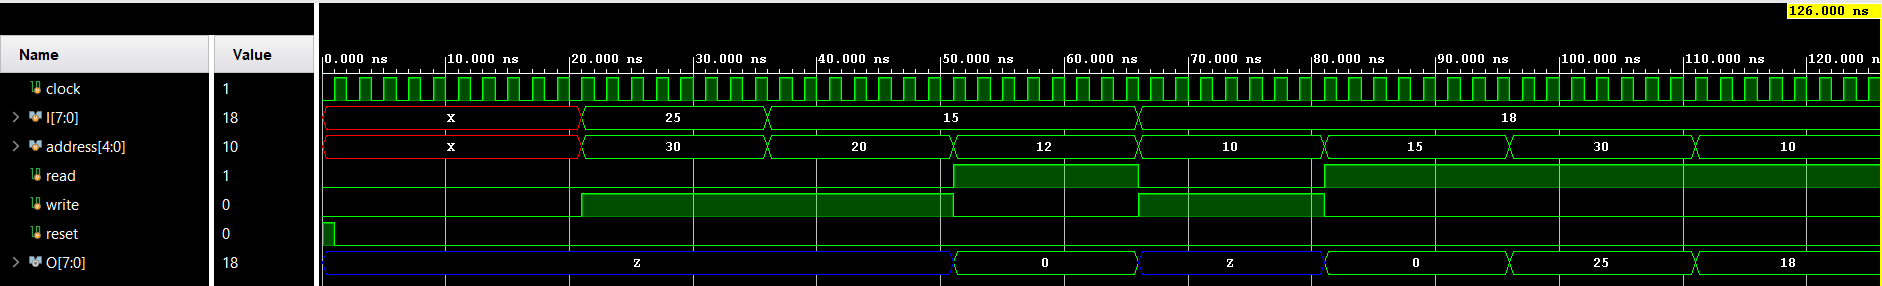
\includegraphics[width=1\textwidth]{simulations/part5_result.png}	
    	\caption{32 byte memory simulation}
    	\label{32 byte memory simulation}
    \end{figure}



\hypertarget{hype6}{}
\subsubsection{PART 6}
\begin{figure}[H]
    	\centering
    	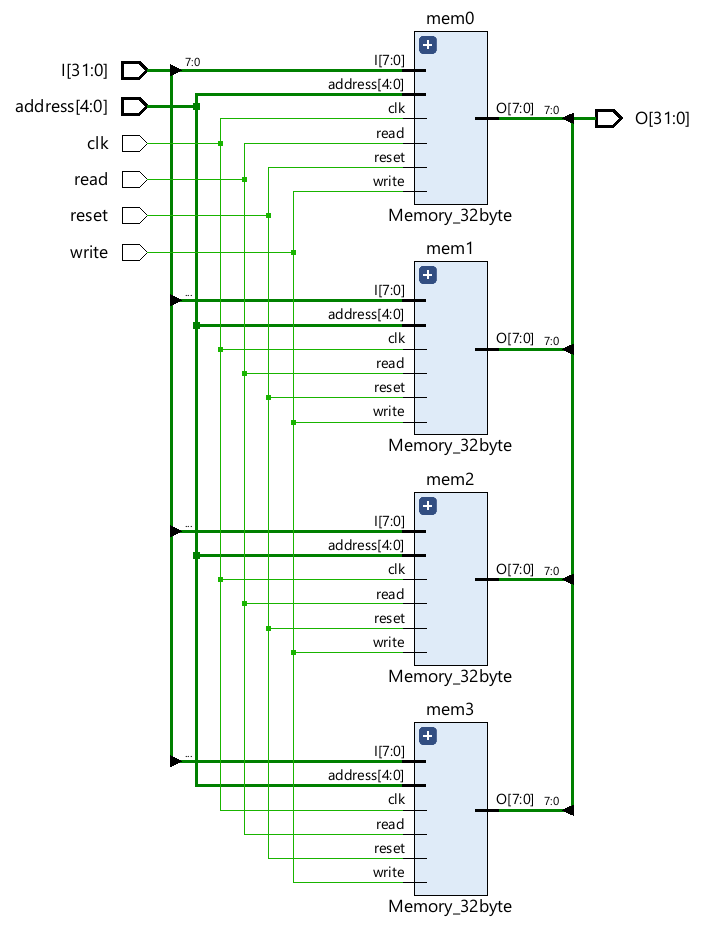
\includegraphics[width=0.8\textwidth]{schematic/part6_design.png}	
    	\caption{128 byte memory}
    	\label{128 byte memory}
    \end{figure}
    
    \begin{figure}[H]
    	\centering
    	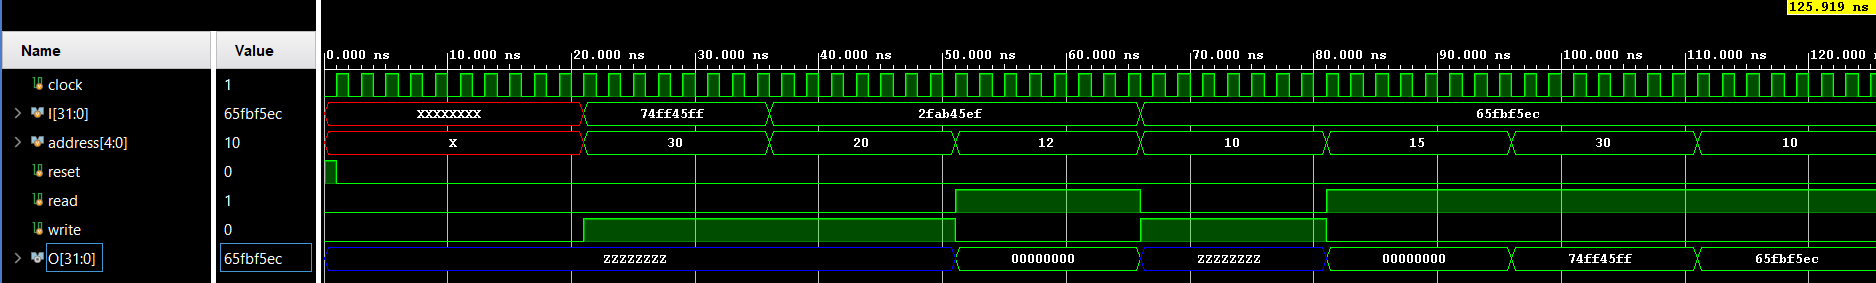
\includegraphics[width=1\textwidth]{simulations/part6_result.png}	
    	\caption{128 byte memory simulation}
    	\label{128 byte memory simulation}
    \end{figure}




\pagebreak

\section{CONCLUSION}
With this homework, we learned how to implement bus without using multiplexers.
At the first question, we designed an three state buffer which we used in many parts.
Then we designed bus with two distinct outputs and inputs.  For the part 3, using 3 different always blocks, we satisfied requirements for the 8-bit memory which has features to manipulate reset, line select, read enable, write enable, and clock inputs. Then using this memory as a line we designed 8 byte memory with 8 rows. In this question we sent 0 as a selector for the address lines that we are not currently using. Then for the 32-bit we separated address into two parts. The most significant 2 bit used for selecting 8 byte memories, whereas other 3 bit memory used for selecting line inside of the chosen 8 byte memory. At the end, we designed an 128 byte memory. There is no need to deactivate any of the 32 byte memories as we totally need 32 bit as input and output, compered to 8 bit input and output of 32 byte memory. We used 4 of them. Overall, all the result and designs gave expected results and satisfied all the requirements for this homework. 


\end{document}

